\chapter{cpMETA: l'Ontolgia di ICOS}
\label{chap:cpMETA}

\section{Panoramica di cpMETA}
\label{section:panoramica}
L'ontologia CPMeta è utilizzata per
la descrizione dei metadati dei dati raccolti
dalle stazioni di monitoraggio ICOS, in particolare
per quanto riguarda la struttura, la qualità e le
informazioni sul contesto di acquisizione dei dati.\\

L'ontologia è basata sul linguaggio formale OWL
(Web Ontology Language) e include una serie di classi,
proprietà e relazioni che descrivono i concetti chiave
e le loro interrelazioni. L'ontologia definisce,
ad esempio, le classi di entità come
la stazione di monitoraggio (\textit{Station}) e
il sensore di misurazione (\textit{Sensor}) e le
proprietà che le collegano. Inoltre, l'ontologia ICOS
Carbon Portal include
anche concetti relativi alla gestione dei dati,
come ad esempio le classi relative ai dataset o alle attività
ad essi legate.\\

L'utilizzo di tale ontologia
consente di standardizzare la descrizione dei
dati e dei metadati provenienti dalle stazioni di
monitoraggio ICOS, garantendo l'interoperabilità tra
i dati provenienti da diverse fonti e la condivisione
dei dati tra i ricercatori e il pubblico in generale.\\

\begin{figure}[h!]
    \centering
    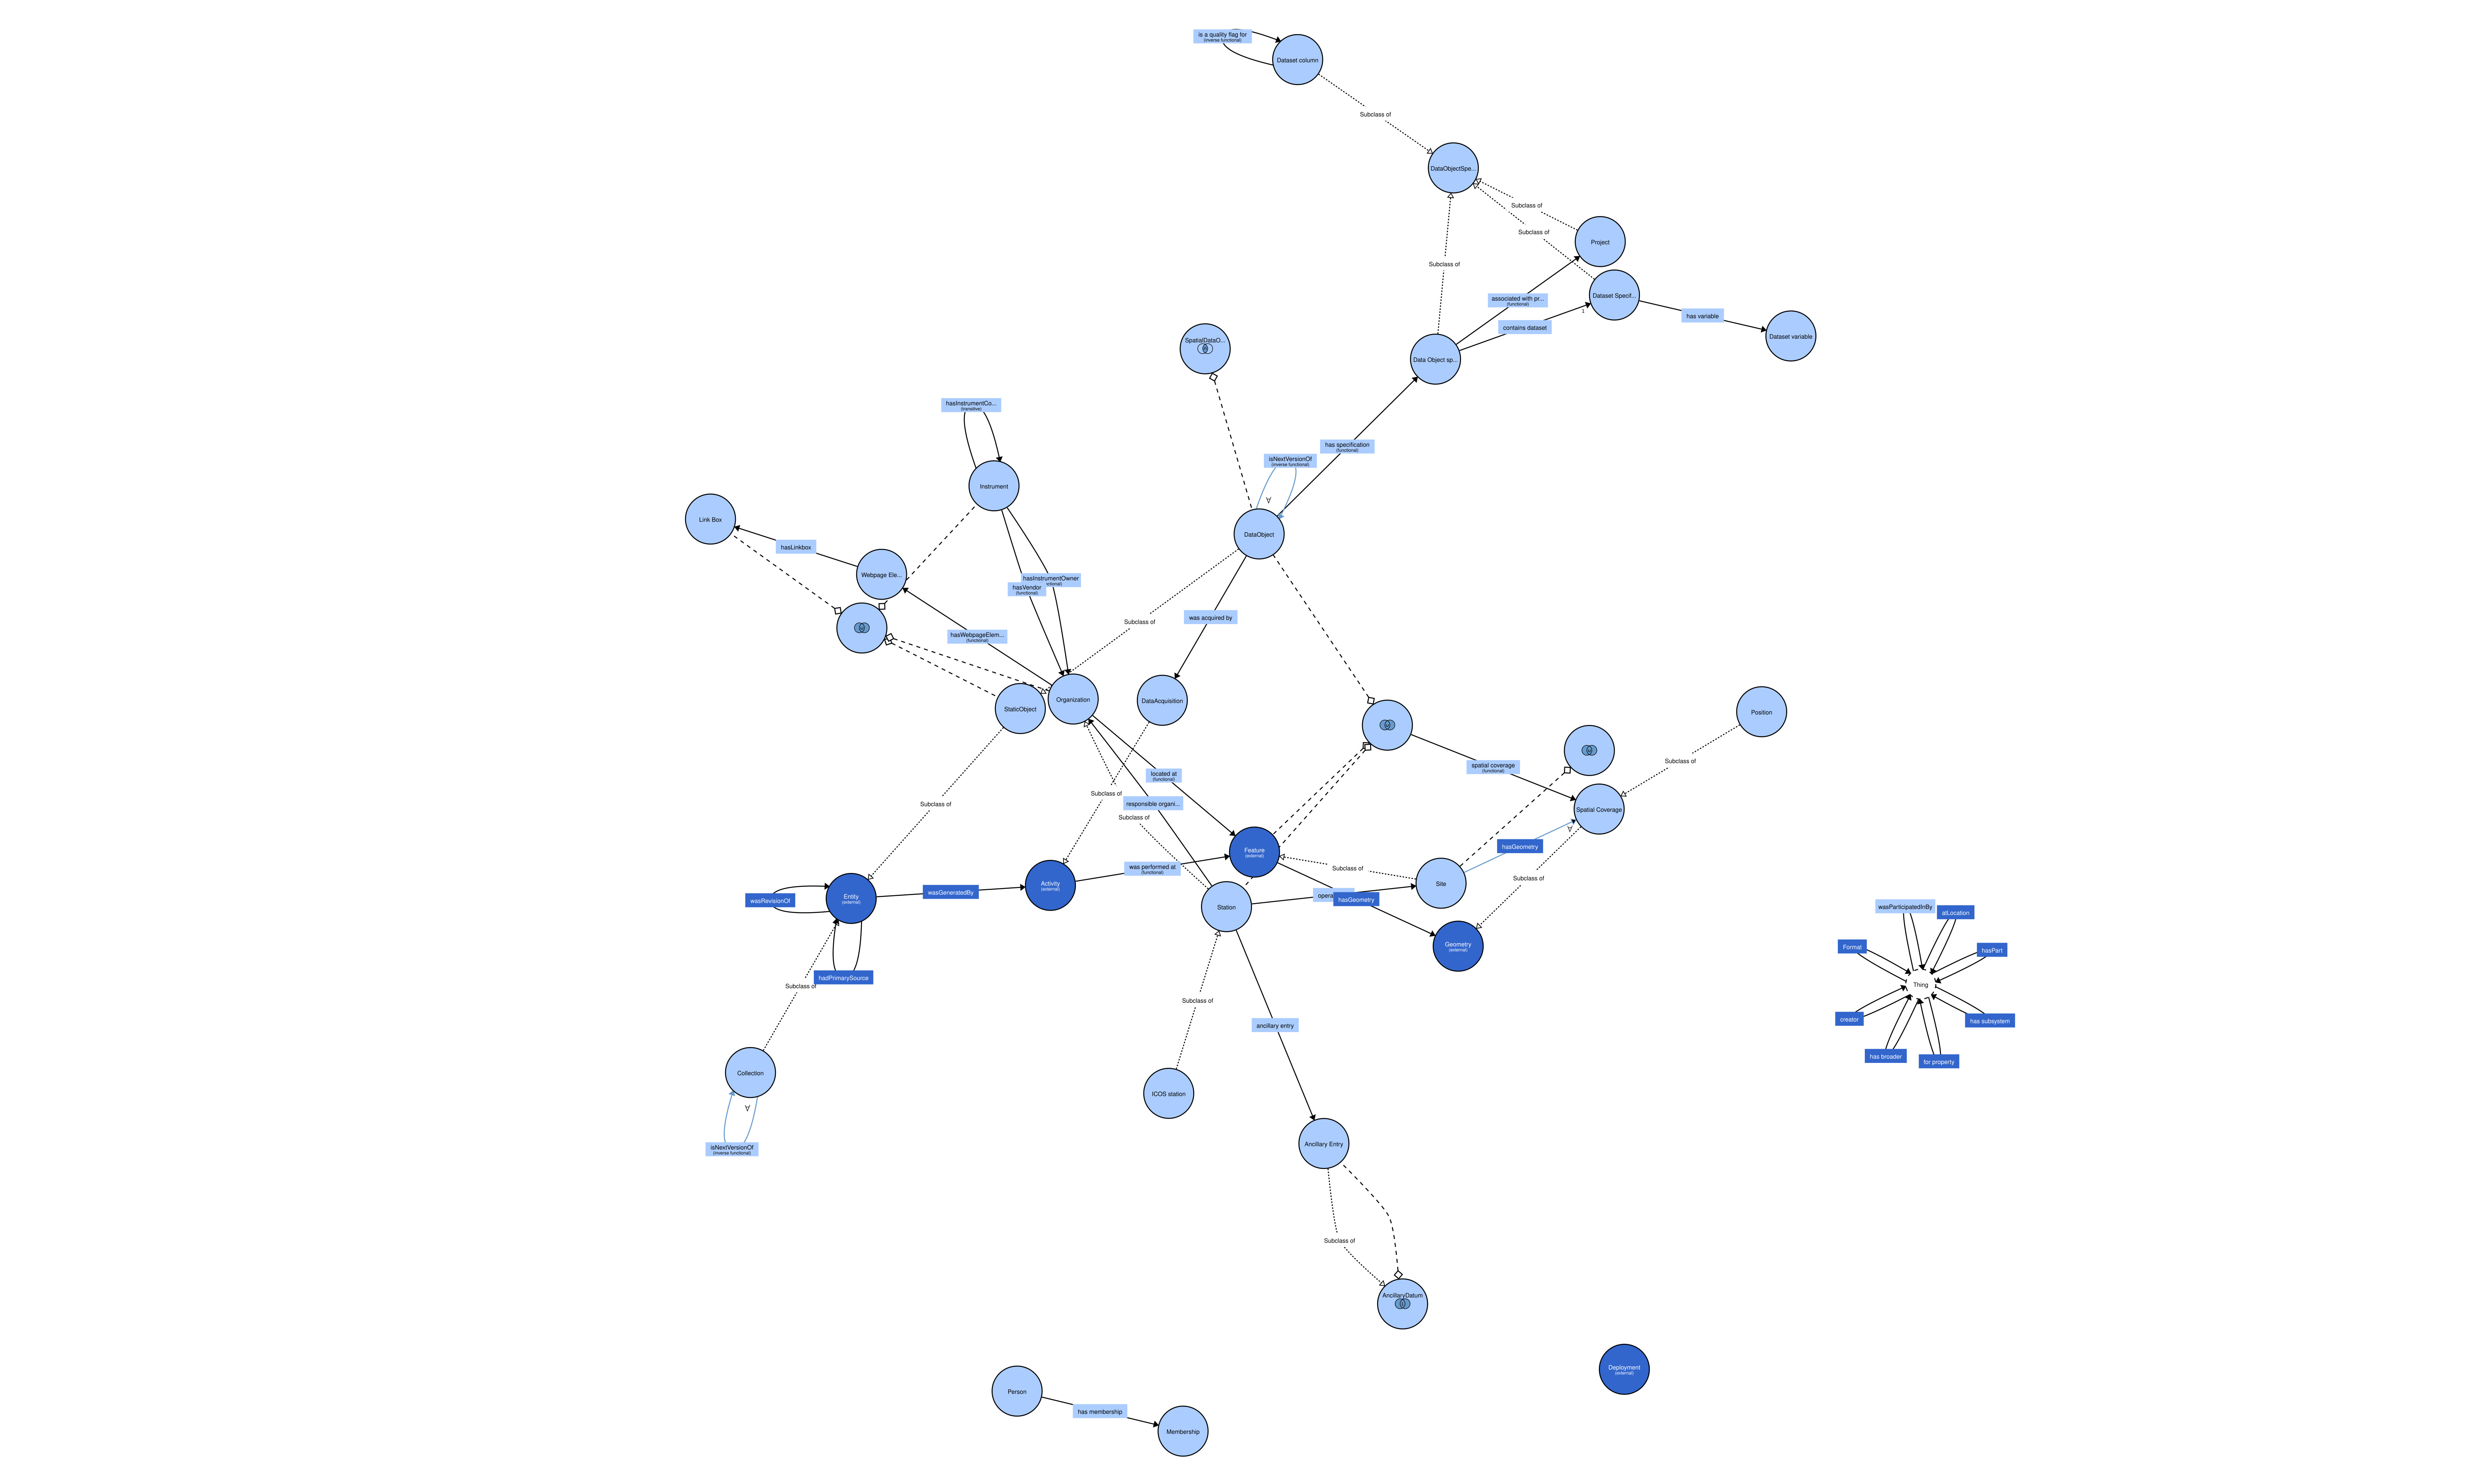
\includegraphics[height=0.6\textwidth]{figures/instanceschema.rdf-_1_.jpg}
    \caption{Struttura di cpMETA.}
    \label{figure:cpmetastructure}
\end{figure}

cpMETA presenta 74 classi e 156 proprietà (63 Object Properties, ovvero
una proprietà che connette un soggetto ed un oggetto con un
predicato, e 93 Data Properties, il predicato connette il
singolo soggetto ad una qualche forma di attributo con un tipo
definito, come string, integer, ecc.). La figura \ref{figure:cpmetastructure}
rappresenta graficamente la struttura dell'ontologia in questione.

\newpage

\section{Esempio di risorsa}
\label{section:esempidirisorse}
Analizziamo ora brevemente uno tra i principali concetti
sviscerati dall'ontologia cpMETA: le stazioni.\\

Le stazioni contengono gli strumenti di misura i cui dati
sono trasmessi al centro di ricerca a cui appartengono,
che provvederà a validare ed elaborare i dati.
Queste stazioni si differenziano a seconda di diversi
parametri tra cui la posizione,
la zona climatica a cui appartengono, il Thematic 
Center a cui fanno riferimento e così via. I metadati
descritti da questo vocabolario OWL per le stazioni di misurazione
sono sintetizzati nelle figure \ref{figure:stationclass} \ref{figure:stationclassgraph} che seguono.

\begin{figure}[h!]
    \centering
    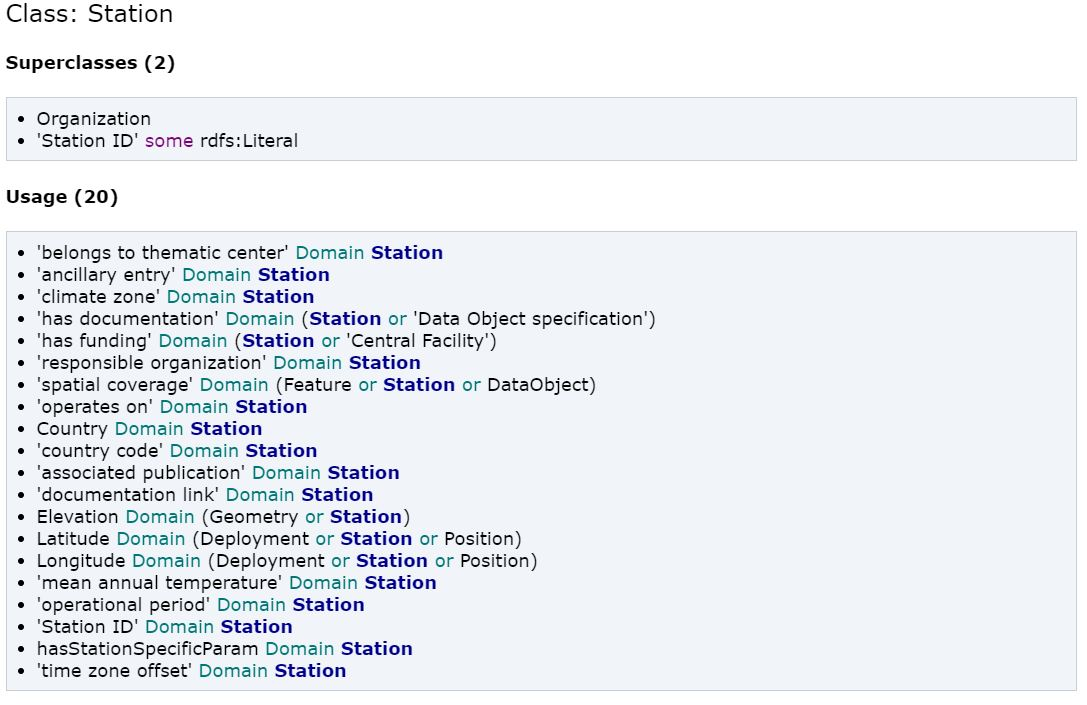
\includegraphics[height=0.6\textwidth]{figures/stationOWL.JPG}
    \caption{Informazioni relative alla classe Station.}
    \label{figure:stationclass}
\end{figure}

\begin{figure}[h!]
    \centering
    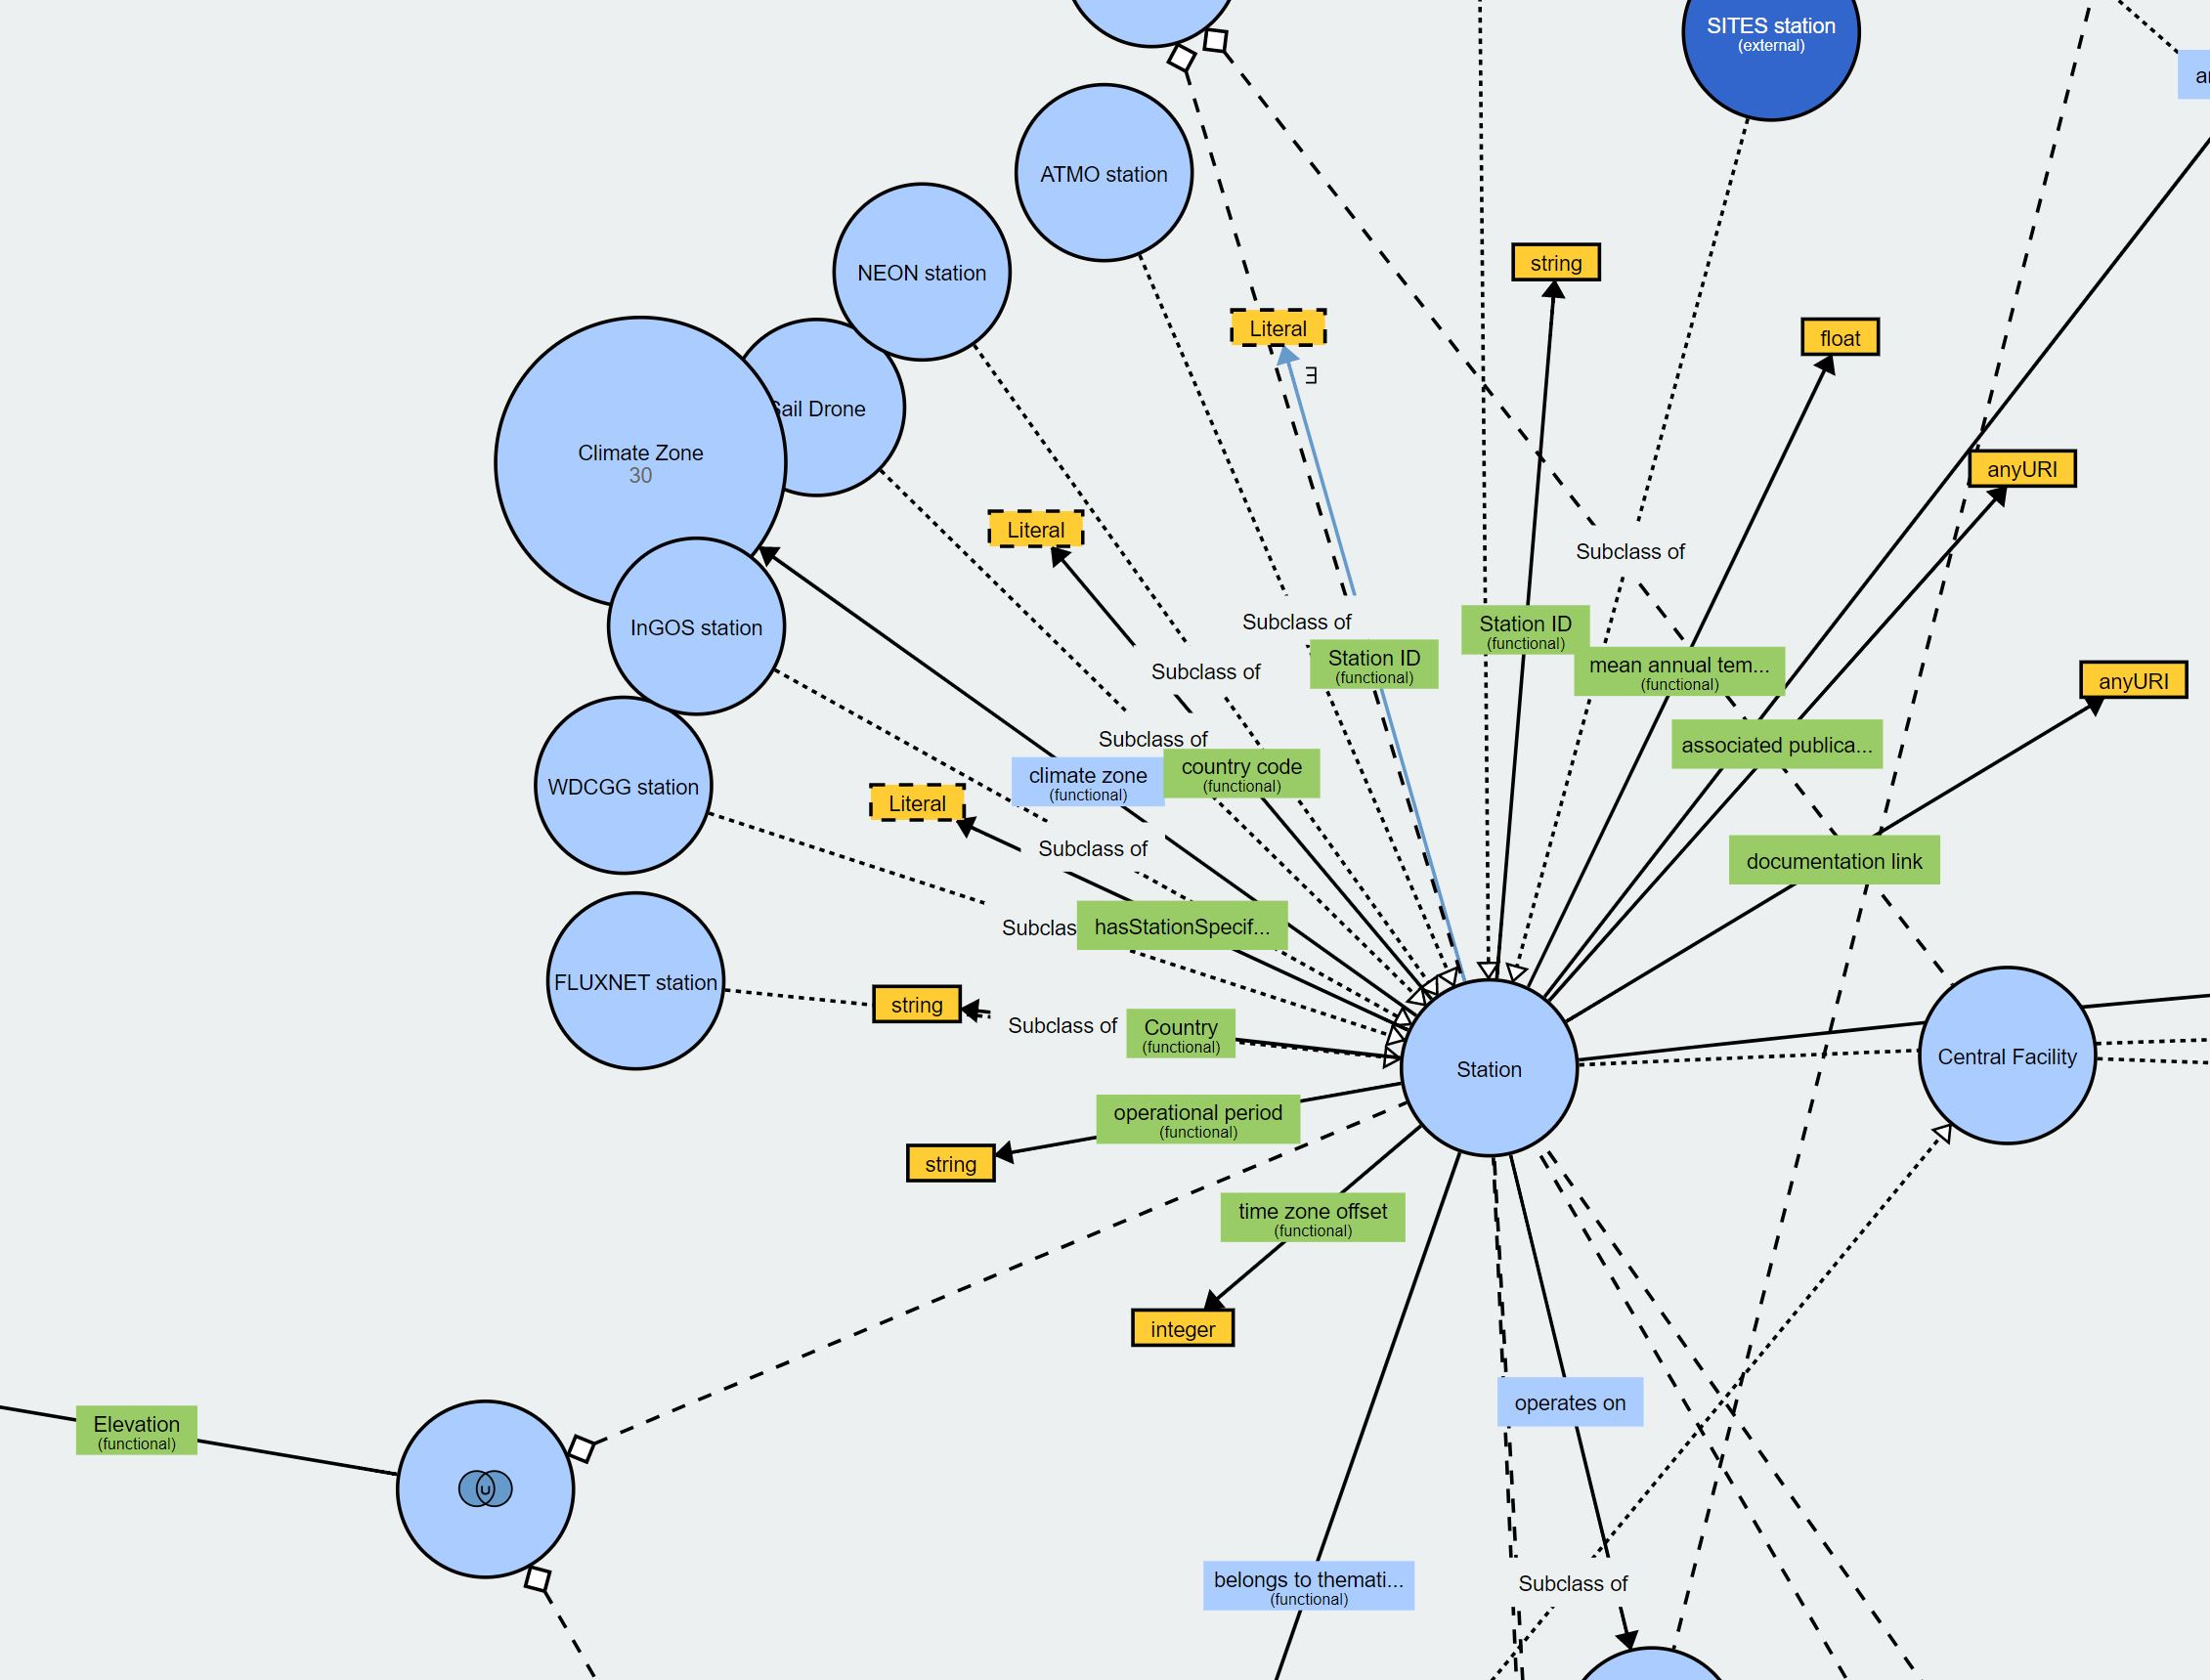
\includegraphics[height=0.6\textwidth]{figures/stationOWLGraph.JPG}
    \caption{Informazioni grafiche relative alla classe Station.}
    \label{figure:stationclassgraph}
\end{figure}

\newpage



\section{Relazioni}
\label{section:relazioni}
In cpMETA le classi sono legate tra loro tramite relazioni. Alcune delle quali sono:
\begin{itemize}
    \item \textit{was performed with}. Lo strumento utilizzato per una certa acquisizione dati.
    \item \textit{has geometry}. Mette in relazione una determinata classe con una latitudine ed una longitudine (rappresentazione spaziale dell'oggetto).
    \item \textit{was performed at}. Relaziona una certa attività (es. acquisizione dati) ad una certa locazione.
    \item \textit{has deployment}. Mette in relazione un certo strumento al suo eventuale deployment vero e proprio.
    \item \textit{has instrumnet owner}. A quale organizzazione appartiene un certo strumento.
    \item \textit{operates on}. Una determinata stazione opera su un certo sito (si intende un sito fisico di ricerca).
    \item \textit{has membership}. Una specifica persona può avere una certa membership per un'organizzazione.
\end{itemize}

\section{Servizi esterni di supporto}
\label{section:ontologiedisupporto}
\begin{itemize}
    \item \textit{PROV}.\\
    
    L'impiego del namespace PROV 
    consente di fornire una rappresentazione formale
    e standardizzata delle informazioni sulla
    provenienza dei dati, che è utile per garantire
    la riproducibilità, la trasparenza e la tracciabilità
    delle analisi e dei risultati scientifici \cite{PROVNamespace}.\\

    Un esempio è la classe \textbf{Entity};
    un'entità è una cosa fisica, digitale,
    concettuale o di altro tipo con alcuni aspetti fissi;
    le entità possono essere reali o immaginarie \cite{PROVEntity}.

    \item \textit{OGC GeoSPARQL}.\\
    
    GeoSPARQL è un protocollo stabilito
    dall'Open Geospatial Consortium (OGC)
    per la gestione e la ricerca di dati
    geografici collegati nel Web semantico \cite{OGCGeoSPARQL}.
    Per facilitare lo scambio di dati geospaziali
    in formato RDF, l'OGC ha definito un'ontologia
    basata su standard ben noti. Questo protocollo
    consente di effettuare ricerche sia qualitative
    che quantitative tramite l'utilizzo del linguaggio
    di query SPARQL.\\

    Un esempio di risorsa GeoSPARQL usata nell'ontologia cpMETA
    è la classe \textbf{Geometry} \cite{OGCGeoSPARQLGeometry}.

    \item \textit{SSN (Semantic Sensor Network) Ontology}.\\
    
    La Semantic Sensor Network (SSN) \cite{SSNOntology}
    è un'ontologia che offre un framework semantico
    per la descrizione dei sensori e delle loro
    osservazioni. Questo framework permette l'integrazione
    e l'analisi dei dati dei sensori in modo coerente e
    comprensibile.\\

    La classe \textbf{Deployment}, descrive la
    distribuzione di uno o più sistemi
    per uno scopo particolare \cite{SSNOntologyDeployment}.


\end{itemize}
